\def\difficulty{3}
\sujet[Color LIP]{Color Logarithmic Image Processing (CoLIP)}
\index{Frameworks!Color Logarithmic Image Processing}

\begin{note}The objective of this tutorial is to have an overview of the Color Logarithmic Image Processing (CoLIP) framework \cite{Gouinaud2013,Gouinaud2011,Gavet2015,Gavet2015a}. The CoLIP is a mathematical framework for the representation and processing of color images. It is psychophysically well justified since it is consistent with several human visual perception laws and characteristics. It allows to consider color images as vectors in an abstract linear space, contrary to the classical color spaces (e.g., RGB and \lab). The  purpose of this tutorial  is to present the mathematical fundamentals of the CoLIP by manipulating the color matching functions and the chromaticity diagram.\end{note}

\vspace*{-.8\baselineskip}

\section{Definitions}
\index{Color!Color Spaces}
This diagram summarizes the transitions between the classical RGB space and the CoLIP space. The transfer matrices are presented in the following.

\resizebox {.8\linewidth} {!} {
  \begin{tikzpicture}
  
      % enrollment - row 1
	\node [block] (LMS) {$(L,M,S)$}; 
	\node [block, right=1cm of LMS] (lms) {$(l,m,s)$};
	\node [block, right=1cm of lms] (lmstilde) {$(\tilde{l},\tilde{m},\tilde{s})$};
	\node [block, below=1cm of LMS] (XYZ) {$(X,Y,Z)$};
	\node [block, below=1cm of XYZ] (RGB) {sRGB: $(R,G,B)$ };
	
	\node [block, below=1cm of lms] (argyb) {$(a,rg,yb)$};
	\node [block, below=1cm of argyb] (chapeau) {$(\hat{a},\hat{rg},\hat{yb})$};
	
	\node [block, below=1cm of lmstilde] (tilde) {$(\tilde{a},\tilde{rg},\tilde{yb})$};
	\node [block, below=1cm of argyb] (chapeau) {$(\hat{a},\hat{rg},\hat{yb})$};
	
	\node [below=.5cm of chapeau,text width=3cm,align=center] (colip){LIP operations:\\
	  $\lipplus{}, \lipfois{}, \lipmoins{}$\\
	  $\lippluschap{}, \lipfoischap{}, \lipmoinschap{}$
	};
	\node [right=1cm of colip,text width=3cm,align=center] {Classical operations};
%  
    % connecting nodes with paths
	\path[dligne] (RGB) -- node[right]{E/2 illuminant} (XYZ);
	\path[dligne] (XYZ) -- node[right]{$\rm{M}_{\rm HPE}$}(LMS);


	\path[dligne] (LMS) -- node[above]{tones} (lms);
	\path[ligne] (lms) -- node[above] {$\varphi$}(lmstilde);
	
	\path[ligne] (lms) -- node[right] {$P\lipfois{scale=1}\cdot$} (argyb);
	\path[ligne] (lmstilde) -- node[right] {$ P\times\cdot$} (tilde);
	\path[ligne] (tilde) -- node[above] {$\varphi^{-1}$} (argyb);
	
	\path[dligne] (argyb) -- (chapeau);
  \end{tikzpicture}
}

\vspace*{-.8\baselineskip}

\subsection{RGB to XYZ}Here, we choose to keep the conventions of the CIE 1931, i.e. a $2^\circ$ 1931 observer, with the equal energy illuminant E and the sRGB space.
Depending on the illuminant, there exist many conversion matrices. 

\begin{mcomment}
\begin{mremark}
	Use \minline{rgb2xyz} function to perform the conversion.
\end{mremark}
\end{mcomment}

\begin{pcomment}
\begin{premark}
Use the module \pinline{skimage.color}.
\end{premark}
\end{pcomment}

% 
% \begin{eqnarray}
% \left(
% \begin{array}{c}
% R\\
% G\\
% B
% \end{array}
% \right)
% =\left( \begin{array}{r@{\hskip 12pt}r@{\hskip 6pt}r}
%                       41.2556 & & \\
%                       21.2758 & & \\
%                       1.9023  & &
%                     \end{array}
% \right)
% \cdot
% \left(
% \begin{array}{c}
% X\\
% Y\\
% Z
% \end{array}
% \right)
% \end{eqnarray}

\subsection{XYZ to LMS}
The matrix $M_{HPE}$ (Hunt, Pointer, Estevez) is defined by:
\begin{eqnarray}
 \left(
\begin{array}{c}
L\\
M\\
S
\end{array}
\right)=
\rm{M}_{\rm HPE}\times
\left(
\begin{array}{c}
X\\
Y\\
Z
\end{array}
\right),
\end{eqnarray}
with

\begin{eqnarray}
\rm{M}_{\rm HPE}=\left( \begin{array}{r@{\hskip 12pt}r@{\hskip 6pt}r}
                     0.38971  & 0.68898 & -0.07868\\
                    -0.22981  & 1.18340 &  0.04641 \\
                     0.00000  & 0.00000 &  1.00000
                    \end{array}
\right).
\end{eqnarray}
\subsection{LMS to lms}\vspace*{-.8\baselineskip}

\begin{equation}
\forall c\in\{l,m,s\}, C\in\{L,M,S\}, c=M_0\left(1-\frac{C}{C_0}\right), 
\end{equation}


with $C_0$ is the maximal transmitted intensity value. $M_0$ is arbitrarily chosen at normalized value 100. Notice that $C\in]0;C_0] $ and $c\in[0;M_0[$.

\subsection{CoLIP homeomorphisme}\vspace*{-.8\baselineskip}
$$\forall f\in S, ~\varphi(f) = -M_0 \textrm{ln}\left(1-\frac{f}{M_0}\right).$$

The logarithmic response of the cones, as in the LIP theory, is modeled through the isomorphism $\varphi$:
\begin{equation}
 \textrm{for }c\in\{l,m,s\},~ \tilde{c}=\varphi(c)=-M_0\ln \left(1-\frac{c}{M_0}\right),
\end{equation}

where $(\tilde{l}, \tilde{m}, \tilde{s})$ are called the logarithmic chromatic tones. 

\subsection{Opponent process}\vspace*{-.8\baselineskip}
\begin{eqnarray}
\left(
\begin{array}{c}
\tilde{a}\\
\tilde{rg}\\
\tilde{yb}
\end{array}
\right)=
P\times
\left(
\begin{array}{c}
\tilde{l}\\
\tilde{m}\\
\tilde{s}
\end{array}
\right),
\end{eqnarray}
 with
\begin{eqnarray}
 P=\left(\begin{array}{c@{\hskip 12pt}c@{\hskip 12pt}c}
          40/61 &20/61 &1/61\\
          1     &-12/11&1/11 \\
          1/9   &1/9   &-2/9
         \end{array}
 \right).
 \label{eq:P}
\end{eqnarray}

\subsection{Bounded vector space}
Three channels $\h{f}=(\hat{a}, \hat{rg}, \hat{yb})$ are defined by:
\vspace*{-.8\baselineskip}
\begin{eqnarray}
  \h{a} &=&a\\
  \h{rg} &=&\left\{
    \begin{array}{cll}
        rg &\textrm{ if }& rg\geq 0\\
        -\lipmoins{} rg &\textrm{ if }& rg< 0
    \end{array} 
  \right. \\
  \h{yb} &=&\left\{
    \begin{array}{cll}
        yb &\textrm{ if }& yb\geq 0\\
        -\lipmoins{} yb &\textrm{ if }& yb< 0
    \end{array} 
  \right.
\end{eqnarray}

\section{Applications}
\subsection{CMF}\index{Color!Color Matching Functions}
\begin{qbox}
Represent the classical chromaticity by using the color matching functions.
\end{qbox}
\begin{mcomment}
\begin{mremark}
	The color matching functions in the different spaces, as well as the wavelength and the purple line, are provided in the matrix \minline{'cmf.mat'}.
\end{mremark}
\end{mcomment}

\begin{pcomment}
\begin{premark}
The color matching functions in the different spaces, as well as the wavelength and the purple line, are provided in the matrix \pinline{'cmf.npz'}. Load it with \pinline{numpy.load}.
\end{premark}
\end{pcomment}

\newpage
\subsection{CoLIP chromaticity diagram}
\index{Color!Chromaticity diagram}
\begin{qbox}
Represent the chromaticity diagram in the plane $(\h{rg},\h{yb})$ as well as the Maxwell triangle of the RGB colors, as in Fig.\ref{fig:rgyb}.
\end{qbox}

\begin{figure}[h]
\centering
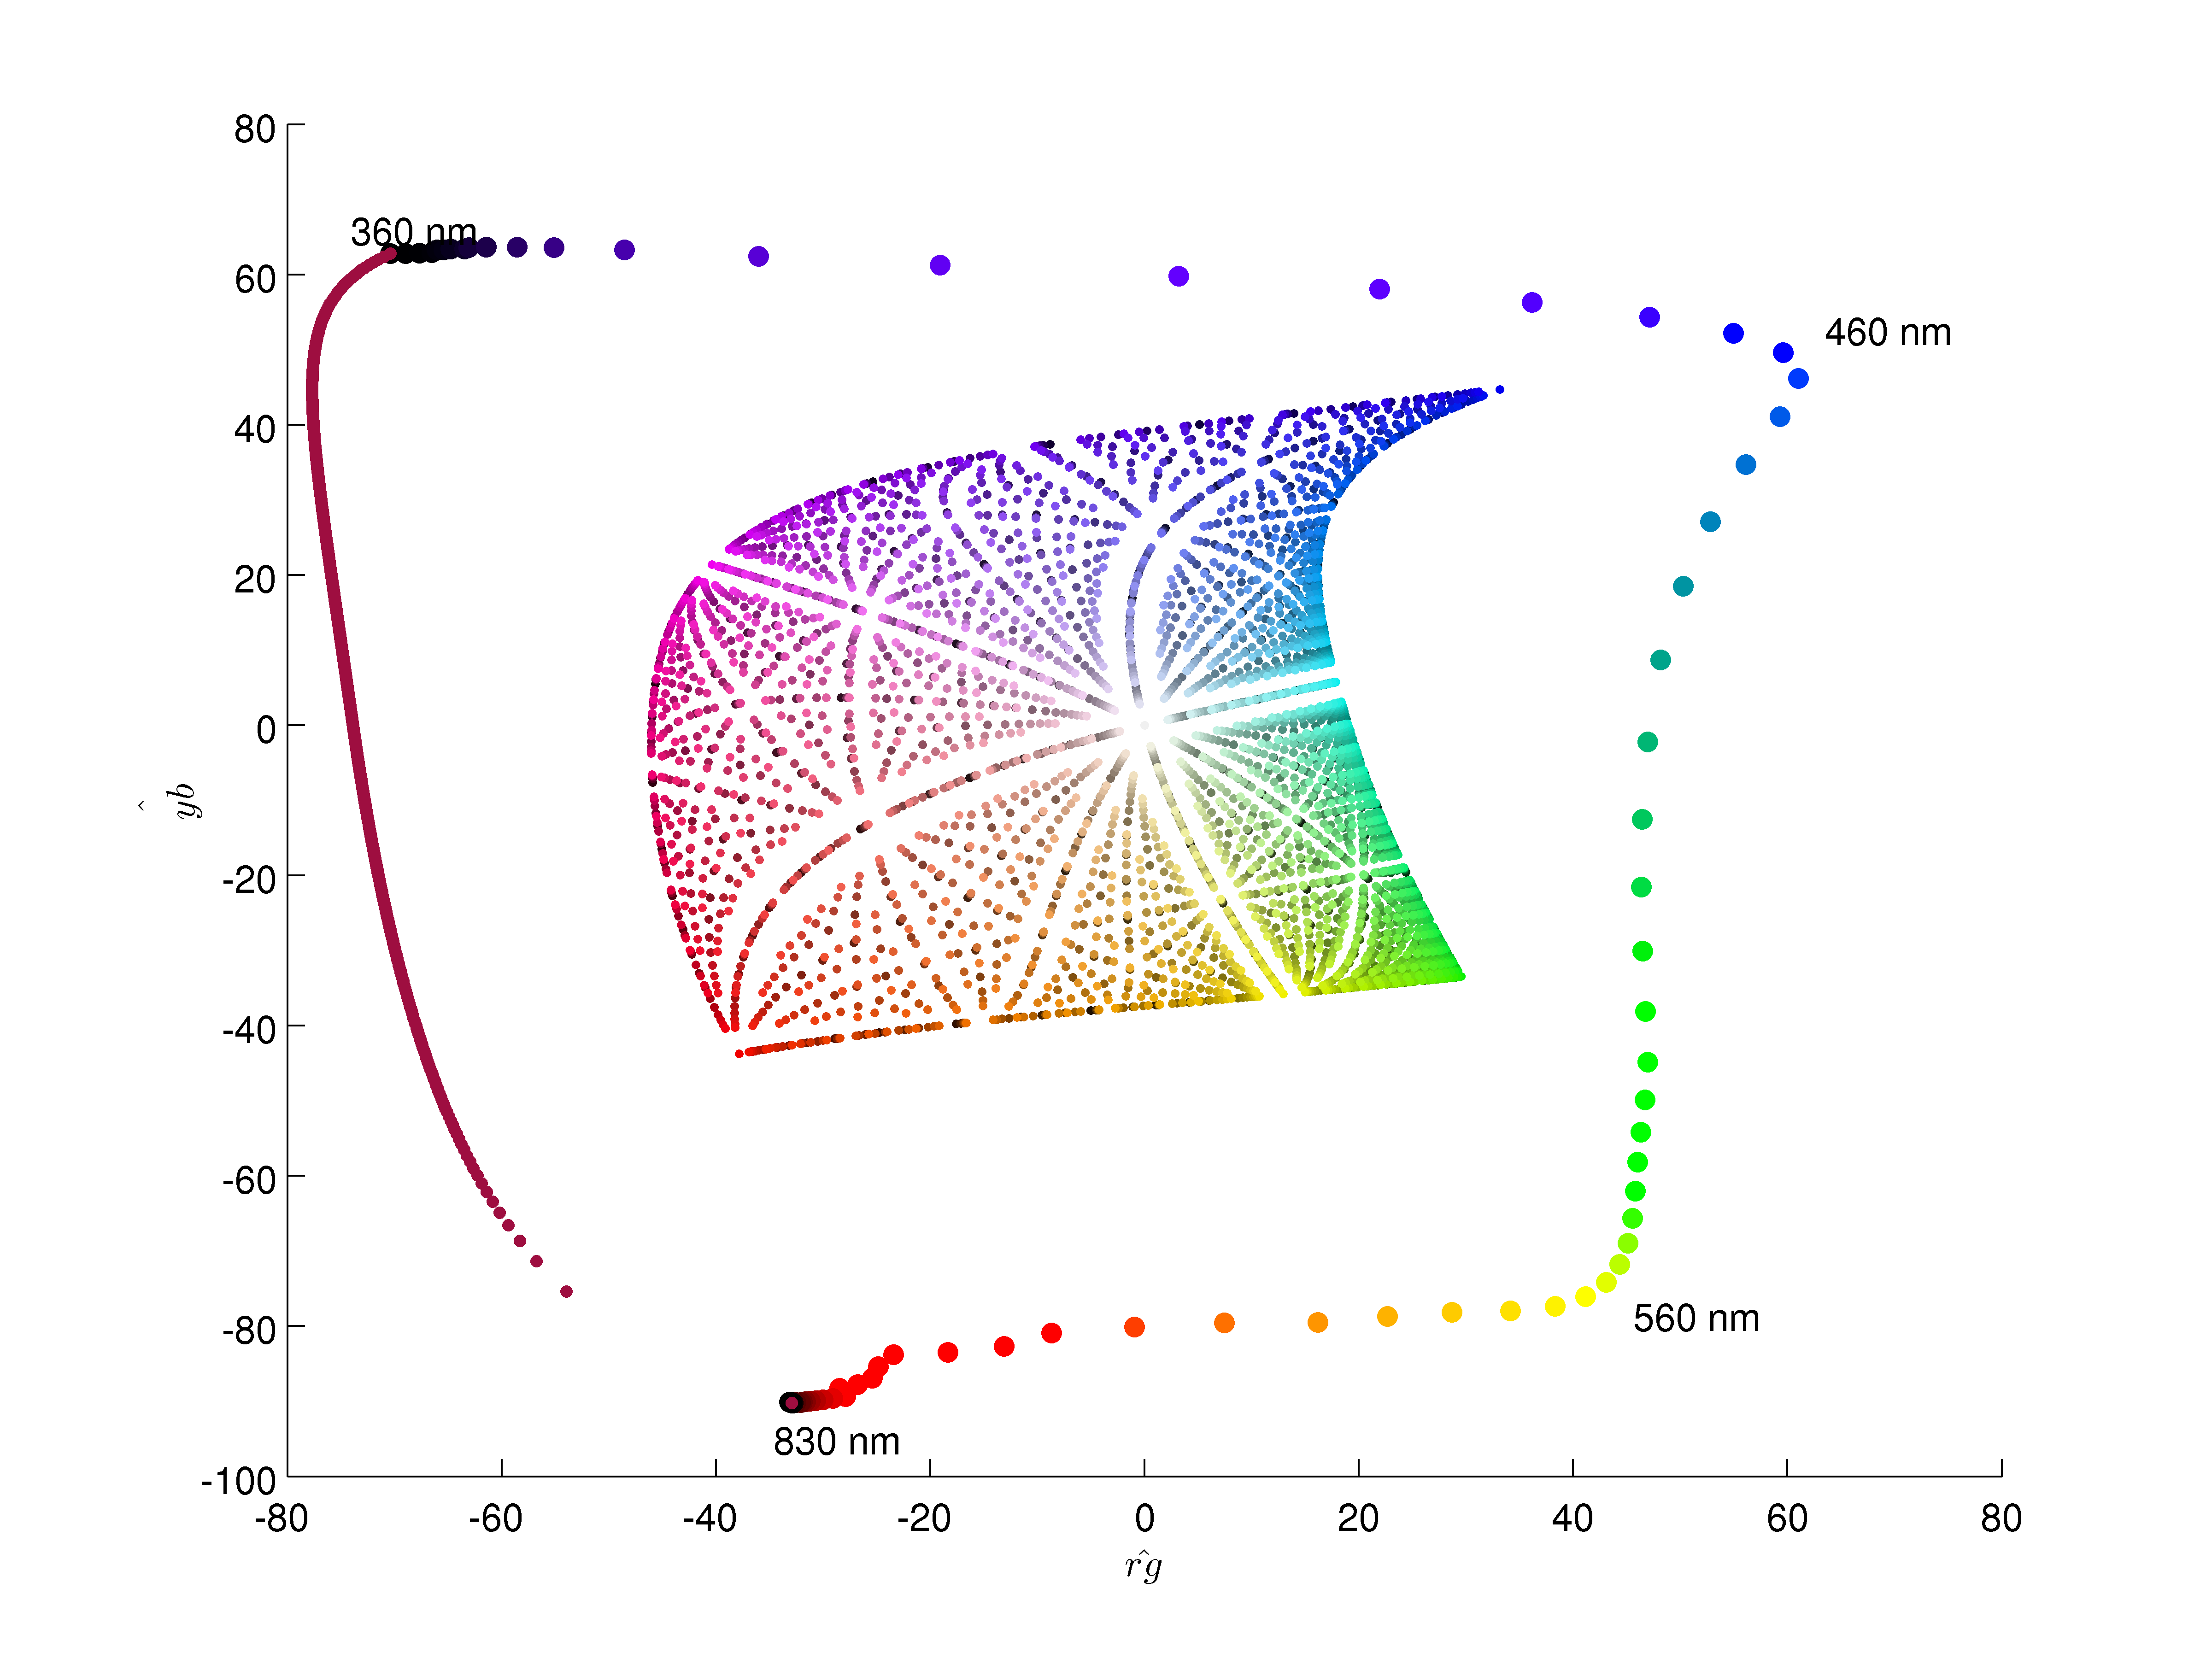
\includegraphics[width=10cm]{chap_chromaticity.png}
\caption{Chromaticity diagram in the plane $(\h{rg},\h{yb})$.}
\label{fig:rgyb}
\end{figure}
